\documentclass[a4paper, 12pt]{article}
\usepackage[utf8]{inputenc}
\usepackage[T1]{fontenc}
\usepackage[serbian]{babel}
\usepackage{amsmath}
\usepackage[margin = 2cm]{geometry}
\usepackage{graphicx}
\usepackage{nopageno}
\usepackage{blindtext}
\usepackage{tabularx}
\usepackage{multirow}
\usepackage{subcaption}
\usepackage{cprotect}
\usepackage{multicol}


\newcolumntype{R}{>{\raggedleft\arraybackslash}X}
\newcolumntype{C}{>{\centering\arraybackslash}X}

\graphicspath{ {./img/} }

\pagestyle{empty}
\newcommand{\btmline}{
\vfill
\rule{0.9\textwidth}{0.4mm}
\begin{center}
13E043RE - Računarska elektronika
\end{center}}

\title{
\Large{Univerzitet u Beogradu - Elektrotehnički fakultet}\\
\vspace{0.5cm}
\large{Katedra za elektroniku}\\
\vspace{1.2cm}
\begin{figure}[h!]
\centering

\includegraphics[scale=1.2]{logo}
\end{figure}
\vspace{3cm}
\Huge{\textbf{\textit{Huffman Coding}}} \\
\vspace{0.5cm}
\Large{\textbf{Implementacija u MASM asemblerskom jeziku}}\\
\vspace{2cm}
\Large{13E043RE - Računarska elektronika}\\
\vfill
}
\author{Radomir Vranjevac 2017/0103\\Dušan Ilić 2017/0070}
\date{}


\renewcommand{\arraystretch}{1}
%==========================================================================
\begin{document}
%==========================TITLE===========================================
\maketitle
\newpage
%==========================================================================
%==========================CONTENTS========================================
\tableofcontents
\newpage
%==========================================================================

\section*{Zadatak}
\addcontentsline{toc}{section}{Zadatak}
Potrebno je napisati program u \textbf{MASM} jeziku koji vrši \textit{Huffman}-ovo kodovanje simbola. Ovo
kodovanje zasnovano je na verovatnoći pojavljivanja simbola gde se simboli sa najvećom verovatnoćom
pojavljivanja koduju sa kodnom rečju najmanje dužine.

Nakon pokretanja programa od korisnika se traži da unese naziv tekstualne datoteke nad kojom želi
da primeni mehanizam \textit{Huffman}-ovog kodovanja. Kao rezultat kodovanja na konzoli se ispisuje
učestanost pojavljivanja pojedinih simbola kao i kodne reči koje su dodeljene pojedinom simbolu.

\btmline\newpage
%==========================================================================

\section*{Uvod}
\addcontentsline{toc}{section}{Uvod}

\textit{Huffman}-ovo kodovanje predstavlja algoritam za kodovanje simbola, gde dužina koda svakog simbola zavisi
od učestanosti ponavljanja datog simbola u određenom tekstu, odnosno tekstualnoj datoteci. Cilj je da se kodovanjem
smanji potreban memorijski prostor za čuvanje sadržaja nekog fajla.

\textit{Huffman}-ovo kodovanje spada u \textit{prefix} kodove, odnosno zadovoljava pravilo da nijedan kod nije prefiks nekog drugog koda
(kodovi u kojima je svaki simbol predstavljen istim brojem bita automatski zadovoljavaju pravilo prefiksa).
Ovo predstavlja dobru osobinu jer znatno olakšava dekodovanje.

U daljem tekstu težićemo da detaljno pojasnimo postupak kodovanja.

\subsection*{Struktura projekta}
\addcontentsline{toc}{subsection}{Struktura projekta}

Prilikom izrade projekta, projekat je podeljen na logičke celine. Ceo projekat se sastoji iz sledećih delova i fajlova:

\begin{enumerate}
\item \textbf{Konfiguracija} - sadrži fajl u kojem se nalaze definicije konstanti i parametara korišćenih u projektu, poput maksimalne dužine niza itd.
	\begin{itemize}
	\item \verb|configuration.inc|
	\end{itemize}
	\item \textbf{Složene strukture} - sadrži fajl u kojem se nalaze definicije složenih struktura podataka koje su korišćene prilikom izrade projekta.
	\begin{itemize}
	\item \verb|structures.inc|
	\end{itemize}
\item \textbf{Rad sa tekstualnom datotekom} - sadrži fajlove za deklaracije i definicije procedura korišćenih za obradu sadržaja tekstualne datoteke.
	\begin{itemize}
	\item \verb|file_process.inc|
	\item \verb|file_process.asm|
	\end{itemize}
\item \textbf{Formiranje \textit{Huffman}-ovog stabla i rad sa njim} - sadrži deklaracije i definicije procedura korišćenih za rad sa \textit{Huffman}-ovim stablom.
	\begin{itemize}
	\item \verb|huffman_tree.inc|
	\item \verb|huffman_tree.asm|
	\end{itemize}
\item \textbf{Glavni program} - sadrži glavni program koji koristi sve pomoćne procedure definisane u ostalim fajlovima.
	\begin{itemize}
	\item \verb|main.asm|
	\end{itemize}
\end{enumerate}

\btmline\newpage
%==========================================================================

\subsubsection*{\textit{Include} fajlovi}
\addcontentsline{toc}{subsection}{\textit{Include} fajlovi}

Svaki \verb|.inc| fajl zaštićen je od višestrukog uključivanja u projekat definisanjem makroa, čije se postojanje proverava prilikom uključivanja u projekat.
Primer koda koji ovo obezbeđuje prikazan je u nastavku.

\begin{verbatim}
ifndef _FILENAME_INC_
_FILENAME_INC_ = 0

	; content goes here
	
endif
\end{verbatim}

\subsubsection*{Strukture podataka}
\addcontentsline{toc}{subsection}{Strukture podataka}

Grafički prikaz struktura koje su korišćene prikazan je na slici \ref{struct}. 

\begin{figure}[h!]
\centering
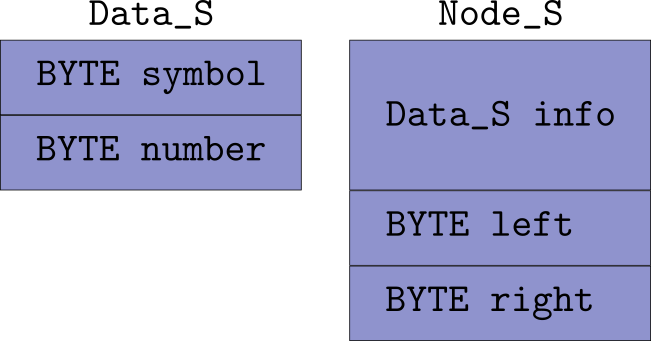
\includegraphics[width=.5\textwidth]{structures}
\caption{Strukture podataka}
\label{struct}
\end{figure}

Polje \verb|symbol| strukture \verb|Data_S| sadrži karakter, a polje \verb|number| sadrži njegov broj ponavljanja.
Struktura \verb|Node_S| predstavlja čvor u \textit{Huffman}-ovom stablu . Polja \verb|left| i \verb|right| koriste se 
za određivanje deteta datog čvora. Detaljnije o ovome u nastavku.

\btmline\newpage
%==========================================================================

\section*{Rad sa datotekom}
\addcontentsline{toc}{section}{Rad sa datotekom}

Deklaracaije procedura za rad sa datotekom su nalaze u fajlu \verb|file_process.inc|. U njemu su navedene deklaracije 5 procedura koje će detaljnije biti opisane u nastavku. Definije svih procedura nalaze se u fajlu \verb|file_process.asm|.

\subsubsection*{\textsf{ReadText}}
\addcontentsline{toc}{subsection}{\textsf{ReadText}}

\verb|ReadText| - kao parametre dobija početnu adresu niza na kojoj se nalazi ime datoteke koju treba pročitati, kao i početnu adresu niza u kojem će biti smešten sadržaj datoteke. 

U navedenoj proceduri koristili smo procedure iz \verb|irvine32.lib| biblioteke, i to: 
\begin{itemize}
\setlength\itemsep{0.1em}
\item \verb|OpenInputFile| - za otvaranje datoteke
\item \verb|ReadFromFile| - za čitanje datoteke
\item \verb|CloseFile| - za zatvaranje datoteke
\item \verb|WriteString| - za ispisivanje eventualnih grešaka prilikom izvršavanja
\end{itemize}
Na kraju procedure se u registru \verb|eax| smešta broj pročitanih karaktera.

\subsubsection*{\textsf{Count}}
\addcontentsline{toc}{subsection}{\textsf{Count}}

\verb|Count| - kao parametre dobija početnu adresu niza na kojoj se nalazi tekstualni sadržaj, dužinu tekstualnog sadržaja, kao i početnu adresu pomoćnog niza koji će po izvršavanju procedure sadržati broj ponavljanja svih \verb|ascii| karaktera u tekstualnom sadržaju.

Osnovna ideja je bila koristiti \verb|ascii| kod svakog karaktera kao indeks niza, i inkrementirati element niza prilikom svakog nailaska na određeni karakter. Vremenska složenost ovog algoritma je minimalna, a ne zahteva previše statički alocirane memorije. Algoritam je prikazan na slici \ref{count}

\begin{figure}[h!]
\centering
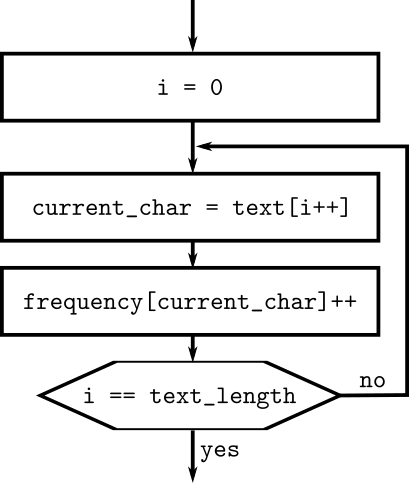
\includegraphics[width=.35\textwidth]{count}
\caption{Algoritam za određivanje broja ponavljanja karaktera}
\label{count}
\end{figure}

\btmline\newpage
%==========================================================================

\subsubsection*{\textsf{Trim}}
\addcontentsline{toc}{subsection}{\textsf{Trim}}

\verb|Trim| - kao parametre dobija početnu adresu niza koji sadrži broj ponavljanja svih \verb|ascii| karaktera u tekstualnom sadržaju, kao i početnu adresu niza koji če po izvršavanju procedure sadržati informaciju o broju ponavljanja karaktera koji se javljaju bar jednom.

Rezultujući niz je niz strukture \verb|Data_S| koja sadrži informaciju o karakteru i njegovom broju ponavljanja. Sve što ova procedura radi je da prolazi kroz ulazni niz, i kada naiđe na karakter koji se javlja bar jednom, pravi strukturu i popunjava je odgovarajućim podacima, a zatim dodaje novi element na kraj niza. Takođe, broj takvih karaktera se na kraju procedure čuva u registru \verb|eax|.

\subsubsection*{\textsf{Sort}}
\addcontentsline{toc}{subsection}{\textsf{Sort}}

\verb|Sort| - kao parametre dobija početnu adresu niza tipa \verb|Data_S| koji sadrži informacije o broju ponavljanja svakog karaktera koji se javlja u tekstualnom sadržaju, kao i dužinu datog niza.

Rezultat izvršavanja procedure je neopadajuće sortiran niz, sortiran po broju ponavljanja datog karaktera. Sortiranje je rađeno \verb|bubble sort| algoritmom.

\subsubsection*{\textsf{PrintResults}}
\addcontentsline{toc}{subsection}{\textsf{PrintResults}}

\verb|PrintResults| - kao parametre dobija početnu adresu niza tipa \verb|Data_S| koji sadrži informacije o broju ponavljanja svakog karaktera koji se javlja u tekstualnom sadržaju, kao i dužinu datog niza.
  
Ova procedura nije od značaja za samo funkcionisanje programa, već služi za proveru dobijenih rezultata prilikom testiranja. Rezultat izvršavanja je ispis svkaog karaktera i njegovog broja ponavljanja na konzolu.

U navedenoj proceduri koristili smo procedure iz \verb|irvine32.lib| biblioteke, i to: 
\begin{itemize}
\setlength\itemsep{0.1em}
\item \verb|WriteString| - za ispisivanje niza karaktera
\item \verb|WriteChar| - za ispisivanje jednog karaktera
\item \verb|WriteDec| - za ispisivanje broja
\end{itemize}

\btmline\newpage
%==========================================================================

\section*{Formiranje stabla}
\addcontentsline{toc}{section}{Formiranje stabla}

\btmline\newpage
%==========================================================================

\section*{Dobijanje koda na osnovu stabla}
\addcontentsline{toc}{section}{Dobijanje koda na osnovu stabla}

Postupak za dobijanje koda simbola na osnovu stabla je izuzetno jednostavan. Kod simbola se čuva u pomoćnom nizu. Kretanjem kroz stablo od korenog čvora (\textit{root}) do lista u kome se nalazi simbol dobija se kod, tako što se pri svakom skretanju levo na kod dodaje - \verb|0|, a pri svakom skretanju desno na kod dodaje - \verb|1|. Ovo je ilustrovano sledećim primerom.


\begin{figure}[h!]
\centering
\begin{subfigure}{.45\textwidth}
	\centering
	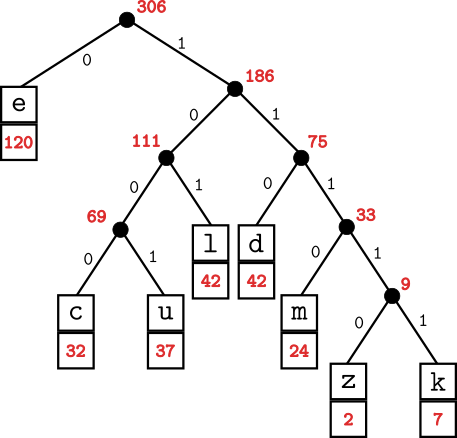
\includegraphics[width=.95\linewidth]{codes}  
	\caption{Primer stabla}
\end{subfigure}
\begin{subfigure}{.45\textwidth}
	\centering
	\begin{tabular}{|c|l|}
	\hline
	\verb|Simbol|	& \verb|Kod|	 \\\hline
	\verb|a|		& \verb|0|		\\\hline
	\verb|b|		& \verb|100|	\\\hline
	\verb|c|		& \verb|101|	\\\hline
	\verb|d|		& \verb|110|	\\\hline
	\verb|e|		& \verb|1110|	\\\hline
	\verb|f|		& \verb|11110|	\\\hline
	\verb|g|		& \verb|11111|	\\\hline
	\end{tabular}
	\caption{Rezultat dekodovanja}
\end{subfigure}
\caption{Primer dobijanja koda na osnovu stabla}
\end{figure}




\btmline\newpage
%==========================================================================

\subsubsection*{Implementacija}
\addcontentsline{toc}{subsection}{Implementacija}

Procedura u kojoj je ovo implementirano deklarisana je u fajlu \verb|huffman_tree.inc|, dok se definicija nalazi u fajlu \verb|huffman_tree.asm|.
Algoritam će biti objašnjen na odabranim delovima koda iz fajla \verb|huffman_tree.asm|.

\vspace{3cm}

\begin{verbatim}
PrintCodes	PROC,\
FirstNode:	PTR Node_S,\	; // First Node pointer 
Dist:		DWORD,\			; // Distance from first element in Nodes array
Code:		PTR BYTE,\		; // Array containing code for a leaf
Index:		DWORD			; // Current index in Code array 
\end{verbatim}

Deo koda iznad predstavlja zaglavlje procedure. \verb|FirstNode| sadrži adresu na kojoj se nalazi prvi čvor u nizu koji sadrži stablo. \verb|Dist| predstavlja udaljenost trenutnog čvora od prvog elementa u nizu. Pri prvom pozivu procedure, ovaj parametar pokazuje na kraj niza, gde je smešten koreni čvor (\textit{root}). \verb|Code| sadrži adresu pomoćnog niza koji čuva kod. \verb|Index| predstavlja indeks u pomoćnom nizu \verb|Code|, ukazuje na sledeću lokaciju za upis.

\vspace{2cm}

\begin{verbatim}
; // Initializing registers
; // esi - pointer to current node
; // edi - pointer to char in string that holds the code
mov		esi, DistBytes
add		esi, FirstNode
mov		edi, Code
add		edi, Index

; // Incrementing index
mov		ecx, Index
inc		ecx
\end{verbatim}

Deo koda iznad predstavlja inicijalizaciju registara koji se koriste u proceduri. U registru \verb|esi| nalazi se adresa trenutnog čvora, dok se u registru \verb|edi| nalazi adresa elementa u nizu \verb|Code| u koji se upisuje. U registru \verb|ecx| čuva se indeks narednog elementa pri narednom pozivu procedure \verb|PrintCodes|.

\btmline\newpage
%==========================================================================

\begin{verbatim}
; // Checking if left child exists
mov		al, BYTE PTR[esi + 2]
.IF(al != NUL)
mov		BYTE PTR[edi], '0'
INVOKE	PrintCodes, FirstNode, eax, Code, ecx
.ENDIF

; // Checking if right child exists
mov		al, BYTE PTR[esi + 3]
.IF(al != NUL)
mov		BYTE PTR[edi], '1'
INVOKE	PrintCodes, FirstNode, eax, Code, ecx
.ENDIF
\end{verbatim}

Deo koda iznad služi za jednostavno kretanje kroz stablo. Naime, na početku se proverava da li postoji levo dete trenutnog čvora. Ako postoji, na kod se dodaje \verb|0|, a zatim se ponovo poziva ista procedura za to levo dete. Ako ovo nije ispunjeno isto se radi za desno dete, s tim što se u slučaju postojanja na kod dodaje \verb|1| . Kao što se može videti, ovde je korišćena rekurzija, pa je izuzetno važno sačuvati registre na stek na početku procedure.

\vspace{2cm}

Nakon ovoga se na kod dodaje karakter za kraj stringa - \verb|'\0'|. Kod koji je smešten u \verb|Code| štampa se jedino ako trenutni čvor predstavlja list u stablu.

\btmline\newpage
%==========================================================================

\section*{Uputstvo za korišćenje programa}
\addcontentsline{toc}{section}{Uputstvo za korišćenje programa}

Program se vrlo jednostavno koristi. Nakon pokretanja korisnika dočekuje prozor prikazan na slici \ref{startup}. Program zahteva ime tekstualne datoteke nad kojom će biti izvršeno \textit{Huffman}-ovo kodovanje. Nakon unosa imena datoteke, pritiskom na \verb|ENTER| započinje izvršavanje programa. Program ispisuje rezultate na konzoli. Primer ispisa rezultata se nalazi na slici \ref{done}. Za kraj izvršavanja programa treba ponovo pritisnuti \verb|ENTER|.

\begin{figure}[h!]
\centering

\includegraphics[width=.5\textwidth]{blank}
\caption{Konzola nakon pokretanja programa}
\label{startup}
\end{figure}

\begin{figure}[h!]
\centering

\includegraphics[width=.5\textwidth]{blank}
\caption{Primer ispisa rezultat nakon završenog kodovanja}
\label{done}
\end{figure}


\end{document}